\chapter{Tutorial on factor graph state estimation}
\minitoc

Let us explicit the terms prevent in this chapter's title. 

The \textit{state} of the robot is a reduced set of variables of particular interest to the roboticist, be it for control, parameter identification, etc.
Those quantities may not directly measurable, due to their physical nature (the center of mass is a virtual point) or because sensor data
is too noisy, biased, or impractical to obtain (\eg GPS for localization is bad close to flat surfaces because of beam reflections). 
Those latent variables can however be estimated by fusing multiple sensors data using a state estimator (aka. observer in automation). 
The task of \textit{estimation} can then simply be stated as finding the most likely robot state given these measurements. 

Probabilistic theory applied to signal processing and information theory has been the bedrock of the state estimation theory development.
In the context of a probabilistic estimator, states are random variables, which, in the robotics context, are mostly continuous. 
The goal is then to find the probability density of those states.
Taking the Bayesian perspective, the most general problem is to find a distribution over a collection of random variables $\cX$ given a set 
of measurements $\cZ$, $p(\cX | \cZ)$, which is known as the \textit{posterior} distribution. 
The Bayes law represents this exact inference:
%
\begin{equation}
    p(\cX | \cZ) = \frac{p(\cZ | \cX) p(\cX)}{p(\cZ)}.
\end{equation}
%
$p(\cZ | \cX)$ is the measurement model that can be obtained through modeling, also called the \textit{likelihood} of the observation. 
$p(\cX)$ is a \textit{prior} that we have on the state variable distribution. This may include for instance knowledge about the initial state of the robot or
an approximate value of parameters that we seek to estimate.
The \textit{marginalized likelihood} $p(\cZ) = \int p(\cZ|\cX)p(\cX)d\cX $ can be thought of as a global normalization constant (\cite{koller2009probabilistic}, chapter 20 ) in case 
the $\cZ$ random variable is observed, which is our case. In general, this term is computationally intractable to compute, since it requires marginalizing
the likelihood distribution over all possible states. Exact inference is therefore rarely possible, the Bayesian practitioner instead relying on approximate inference methods.

In the context of robotics, recursive Monte Carlo sampling (\cite{koller2009probabilistic}, chapter 11) has been 
leveraged in the popular recursive particle filter for tasks such as localization \cite{dellaert1999monte} and SLAM \cite{montemerlo2002fastslam}. A very interesting
property of this approximation is the fact that multimodal distributions can be modelled, which can be useful
for multihypothesis problems such as the kidnapped robot problem \cite{dellaert1999monte} or target tracking \cite{gustafsson2002particle}. 

Application of variational inference (\cite{koller2009probabilistic}, chapter 11) is scarcer. The idea here is to search for a candidate distribution 
(usually a Gaussian) that minimizes the Kullback-Leibert divergence between the posterior and the candidate distribution. Very recent works start 
to find applications in robotics as alternative to MAP-based graph optimization \cite{barfoot2020exactly, wong2020variational} 
or to Bayes filtering \cite{lambert2022recursive}. 

A more popular approach to the estimation problem is to find the mode of the mode of the posterior distribution, aka. the \textit{Maximum A Posteriori} (MAP).



\section{Maximum A Posteriori estimation}

An efficient way to characterize the posterior distribution is to first find its mode, that is the states that 
result in the highest posterior probability. The estimation problem is, in this case, a unconstrained optimization problem
%
\begin{equation}
    \label{eq:MAP_pbe}
    \cX^{MAP} \triangleq \argmax_{\cX} p(\cX | \cZ) = \argmax_{\cX} p(\cZ | \cX) p(\cX).
\end{equation}
%

Notice that the $p(\cZ)$ term does not appear anymore on the right side since it is constant with respect to $\cX$.
States variables $\cX$ in our case are a collection of random variables $\{\cX_i\}_{i \in [1..n]}$ that each relate to a physical quantity of 
interest (\eg the initial robot position, constant camera parameters, orientation of an object in the scene, IMU biases, etc.). Measurements $\cZ$ are 
similarly a collection of individual sensor measurements $\{\bfz_i\}_{i \in [1..m]}$.

Additional assumptions have to be made in order to obtain a numerical implementation of this problem.
First, the measurements are supposed to be conditionally independent of each other, so that the likelihood function can be factorized 
%
\begin{equation}
    p(\cZ | \cX) p(\cX) =  p(\cX_{S_0}) \prod_{i=1}^{n} p(\bfz_i | \cX_{S_i}).
\end{equation}
%
Each factor represents the measurement model associated to the  observation $\bfz_i$ and depending only on a subset $S_i$ of the state variables $\cX_{S_i}$. 
$S_0$ denotes the subset of random variables on which we have nonuniform prior.
Secondly, the measurements are assumed to be corrupted by multivariate Gaussian noise:
%
\begin{equation}
    p(\bfz_i | \cX_{S_i}) = \frac{1}{\sqrt{2\pi\Cov_i}} ~ \exp(- \frac{1}{2} (||\bfe_i(\cX_{S_i})||^2_{\Cov_i}) \triangleq K_i~\phi_i(\cX_{S_i})
\end{equation}
%
where the \textit{residuals} $\bfe_i(\cX_{S_i}) \in \Reals^{M_i}$ are (potentially) nonlinear functions of the state variables, $K_i \in \Reals$ are constants, 
$\Cov_i \in \Reals^{M_i \times M_i}$ is the covariance of the observation noise,
$\phi_i(\cX_{S_i})$ is the un-normalized measurement likelihoods called \textit{factors}, and 
%
\begin{equation*}
    ||\bfe_i(\cX_{S_i})||_{\Cov_i} = \sqrt{\bfe_i(\cX_{S_i}) \Cov_i^{-1} \bfe_i(X_{S_i})}
\end{equation*}
%
is known as the squared Mahalanobis distance. 
Residuals $\bfe_i$ can generally be formulated as a difference between a \textit{expectation function} $\bfh$ and the actual measurements
%
\begin{equation}
    \bfe_i(\cX_{S_i}) = \bfh(\cX_{S_i}) - \bfz_i,
    \label{eq:error_expectation}
\end{equation}
%
% where $\ominus$ is a generalized difference operator,
although some exceptions may exist (see for instance the IMU preintegration residual \eqRef{eq:preint_residual} in \secRef{sec:preint_residual}).

Thus, the posterior probability is proportional to a product of individual factors:
%
\begin{equation}
    p(\cX | \cZ) \propto \phi_0(\cX_{S_0}) \prod_{i=1}^{n} \phi_i(\cX_{S_i}) 
    \label{eq:likelihood_factorization}
\end{equation}
%
Recognizing than maximizing the likelihood in \eqRef{eq:MAP_pbe} is equivalent to minimizing the negative log-likelihood.
%
\begin{align}
    \cX^{MAP} 
    &= \argmin_{\cX} - \log p(\cX | \cZ) &\text{\small MAP problem definition}
    \\
    &= \argmin_{\cX} - \log p(\cZ | \cX) p(\cX) &\text{\small Unaffected Partition constant}
    \\
    &= \argmin_{\cX} - \log p(\cX_0) \prod_{i=1}^{n} p(\bfz_i | \cX_{S_i})  &\text{\small Conditional independences}
    \\
    &= \argmin_{\cX} - \log \phi_0(\cX_{S_0}) \prod_{i=1}^{n} \phi_i(X_{S_i}) &\text{\small Factorized likelihood}
    \\
    &= \argmin_{\cX}  \sum_{i=0}^{n} ||\bfe_i(\cX_{S_i})||_{\Cov_i}^2  &\text{\small Gaussian measurement models}
\end{align}

Thus, solving the MAP problem with the aforementioned hypotheses boils down to solving a nonlinear weighted least-squares (NLLS) problem.
Notice that we included the prior in the sum of the residuals, as it is mathematically equivalent to a measurement model even if it conceptually
comes from a different source of information. 
The weights are the inverse of the measurement covariances: the more uncertain a measurement is, the higher its covariance and, therefore, the lower its influence
on the weighted squared residuals sum. 

A vast part of the literature on MAP estimation has been dedicated to the implementation of efficient ad hoc NLLS solvers. Most of them are 
gradient-based algorithm, typically some variation of the Gauss-Newton algorithm, such as the Levenberg-Marquardt algorithm \cite{boyd2004convex}.





%
%
%
%
%
%
%
\section{Gauss-Newton algorithm}
In this section, we will give a brief introduction to a commonly used way to solve the MAP problem expressed as a NNLS: the Gauss-Newton algorithm.
For now, we will assume that state variables and measurements all live in vector spaces to simplify the derivations. For many practical robotics applications,
some state variables such as rotation matrices live in more complex manifolds. The section is based on tutorials such as \cite{dellaert2017factor,sola2017course}. 

\subsection{Derivation of the Gauss-Newton step}
First, we will simplify notations by dropping dependencies on state variables $X_{S_i}$ where evident to lighten notations. 
Secondly, we will make a simple change of variables. The weighted squared residuals can be expressed as:
\begin{equation}
    ||\bfe_i||^2_{\Cov_i} = \bfe_i \Cov_i^{-1} \bfe_i 
    = (\Cov_i^{-\frac{1}{2}}\bfe_i)^T\Cov_i^{-\frac{1}{2}}\bfe_i
    = ||\Cov_i^{-\frac{1}{2}}\bfe_i||^2 = ||\bfr_i||^2
\end{equation}
where $\bfr_i(X_{S_i}) \triangleq \Cov_i^{-\frac{1}{2}}\bfe_i(X_{S_i})$ can be interpreted as a whitened residual. $\Cov_i^{-\frac{1}{2}}$ can be obtained
from the Cholesky factorization of $\Cov_i^{-1}$. Therefore, the NLLS MAP problem can simply be written:

\begin{equation}
    \cX^{MAP} = \argmin_{\cX} \cL(\cX) \triangleq||\bfr||^2 = \sum_i^{i=N} ||\bfr_i({\cX_{S_i}})||^2 
\end{equation}
were $\bfr$ is a vector of vertically stacked residuals (column vectors) and the cost function $\cL(\cX)$ is simply the squared norm 
of the residual vector. Let's assume we have a current estimate of the state variables $\check{\cX}$.
Each residual can be linearized with respect to this estimate:

\begin{equation}
    \bfr_i(\cX_{S_i}) = \bfr_i(\check{\cX}_{S_i} + \Delta \bfx_i) \approx \check{\bfr}_i + \check{\bfJ}_i \Delta \bfx_i
\end{equation}

where $\check{J}_i$ is the jacobian of the residual at $\check{\cX}_{S_i}$: 

\begin{equation}
    \check{\bfJ}_i \triangleq \left.\frac{\partial \bfr_i}{\partial \cX_{S_i}}\right|_{\check{\cX}_{S_i}}
    \label{eq:res_jacobian}
\end{equation}

We can note $N = \sum_{i=1}^{n}dim(\bfx_i)$ and $M = \sum_{i=1}^{m}dim(\bfe_i)$.
We also stack up the $\Delta \bfx_i$ column vectors as $\Delta \bfx \in \Reals^N$ and the residual jacobians at the linearization point 
$\check{\bfJ} \in \Reals^{M \times N}$ so that the linearized cost function writes:  
%
\begin{equation}
    \cL(\check{\cX} + \Delta \bfx) 
    \approx ||\check{\bfr} + \bfJ \Delta \bfx||^2 
    = \check{\cL} +  \check{\bfr}^T \check{\bfJ} \Delta \bfx + \frac{1}{2}\Delta \bfx^T \check{\bfJ}^T \check{\bfJ} \Delta \bfx 
    \triangleq \cF(\Delta \bfx)
\end{equation}.

We now drop the $\check{\cdot}$ notation to lighten notations $\cF(\Delta \bfx)$ is therefore a local parabolic approximation of 
$\cL$ around the current estimate and $\bfH \triangleq \bfJ^T \bfJ$ is the approximate Hessian of $\cL$ 
\footnote{See \cite{sola2017course} Section 4.2.1 for more details on the nature of the approximation.}. Note that by construction, $\bfH$ is always 
semi-definite positive.

The optimal step (Gauss-Newton step) $\Delta \bfx^*$ is found by differentiating $\cF$ with respect to $\Delta \bfx$ and and equaling to 0 
which gives the linear system of equation:
\begin{equation}
    \bfH \Delta \bfx^* = - \bfJ^T \bfr%, \quad \quad \bfA \triangleq \bfH, \quad \quad \bfb \triangleq 
\end{equation}

Substituting $\bfH$ by its expression, the Gauss Newton step is found by solving the linear system, that is to say inverting $\bfH$:

\begin{equation*}
    \Delta \bfx_{GN}^* = - \bfH^{-1} \bfJ^T \bfr = - (\bfJ^T \bfJ) \bfJ^T \bfr = -  \bfJ^{+} \bfr
\end{equation*}
where $\bfJ^{+}$ is the (right) pseudo inverse of the residual gradient. 

In practice, this matrix $\bfJ^{+}$ is not computed explicitly as more efficient linear system exists. In particular methods based on the Cholesky
factorization of $\bfH$ and on the QR factorization of $\bfJ$ are commonly used in SLAM since they are able to exploit the sparsity of these
matrices.

Taking a Gauss-Newton step then refers to applying the optimal step to get a new estimate:

\begin{equation}
    \check{\cX} := \check{\cX} + \Delta \bfx^*
    \label{eq:gaussian_step}
\end{equation}


\subsection{Gauss-Newton algorithm}
The Gauss-Newton algorithm is an iterative algorithm to find the minimum of NLLS cost functions that can be decomposed in a series of steps.
\begin{enumerate}
    \item Initialize the state estimate at an initial value $\check{\cX} := \cX^0$
    \item Approximate the cost function $\cL(\cX)$ around the current estimate as a quadratic function
    \item Find the optimal step $\Delta \bfx^*$ by solving a linear set of equations, as explained above
    \item Update the current state estimate $\check{\cX} := \check{\cX} + \Delta \bfx^*$
    \item Loop over steps 1-3 until convergence
\end{enumerate}




\subsection{Levenberg-Marquadt}
The Gauss-Newton algorithm is only as valid as the quadratic approximation of its cost function is. Close to the optimum, this approximation
is quite good and leads to a quadratic convergence of the optimization procedure. If the current estimate is farther from the optimum and the
local shape of the cost function is flat, that is if the hessian has small eigen values, the resulting step can be too large and lead to a 
divergent behavior. The Levenberg-Marquadt is an extension of the Gauss-Newton algorithm in which the definition of the $\bfA$ matrix is modified
to alleviate this phenomenum.

\paragraph{Levenberg}
Levenberg \cite{levenberg1944method} contribution was to propose to dampen the Hessian by the identity matrix:
%
\begin{equation}
    \Delta \bfx_{L}^* = - \alpha (\bfH^{-1} + \lambda \bfI)^{-1} \bfJ^T \bfr
\end{equation}
%

$\alpha$ and $\lambda$ are scalar coefficient that can be tuned depending on the evolution of the cost function. 
In particular, $\lambda$ controls the amount of damping: for a given $\lambda$ computed step is wrong (the cost function goes up),
$\lambda$ is increased so that the Hessian influence is diminished. For large values, the steps are close to a gradient descent step.
$\alpha$ provides a way to tune the size of the gradient steps.

\paragraph{Marquadt}
Marquadt \cite{marquardt1963algorithm} improves on Levenberg proposition by proposing to dampen not by the Hessian diagonal $\text{diag}(\bfH)$
instead of the identity matrix. The damping affects each direction of the state differently, depending on the local shape of the cost function:
%
\begin{equation}
    \Delta \bfx_{L}^* = - \alpha (\bfH^{-1} + \lambda \text{diag}(\bfH))^{-1} \bfJ^T \bfr
\end{equation}
%

For both cases, the values of $\alpha$ and $\lambda$ are continuously adapted, which can be understood as an implementation of the 
Trust Region paradigm \cite{boyd2004convex}.


For very large structure from motion problems, Conjugate Gradient Descent is also used as an alternative to Gauss-Newton derivates, though extra care has to 
be taken toward the conditioning of the problem Hessian.





\section{Covariance of the estimate}

An important question to ask is how confident are we in our MAP estimate? Even if our priors and measurements models are Gaussian distribution, the posterior distribution
is not in general Gaussian (unless all measurements models are linear). The region near the peak of the posterior is, however, often nearly Gaussian in shape.
The curvature around the mode is described by the Hessian the negative log likelihood of the posterior at the MAP estimated state. 
The Hessian is actually the \textit{information matrix} of the problem, so that finding the covariance of the MAP estimate resolves to inverting a 
sparse positive definite matrix \footnote{The proof of this statement is out of the scope of this document and can be found in Section 5.1 of 
\cite{peng2018advanced}}. This Hessian is immediately related to Hessian of the residual vector norm by a factor 2 since:

\begin{equation*}
    -\log p(\cX|\cZ) = cst + \frac{1}{2}\cL(\cX)
\end{equation*}

This way, we can approximate our posterior by a multivariate Gaussian, which mean is the mode value and covariance 
is the problem hessian inverse. 

\begin{equation}
    p(\cX | \cZ) \approx \text{Gauss}(\cX^{MAP}; 2\bfH^{-1})
    \label{eq:map_laplace}
\end{equation}

This referred to as the Quadratic or Laplace approximation (\cite{mcelreath2018statistical}, section 2.4.2). MAP inference is then a two step process: 
first find the mode of the posterior (the MAP), then "fit a Gaussian" on this mode. 
To contrast this approach with aforementioned approximations, variational inference as applied in Barfoot et al. 
 \cite{barfoot2020exactly} for instance fit both the mean an the covariance of a Gaussian model as a result of a single optimization problem.

 We can illustrate the Laplace approximation with a one dimensional toy problem (borrowed from Barfoot \cite{barfoot2017state}, section 4.1.1).

 \begin{figure}[h]
    \centering
    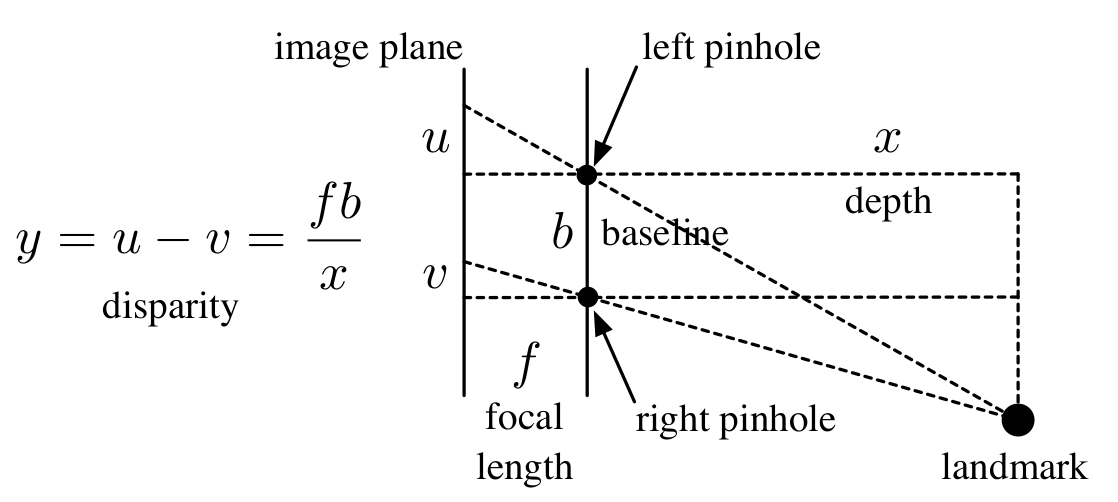
\includegraphics[width=0.6\textwidth]{figures/barfoot_stereo.png}
    \caption{Stereo depth estimation toy model \cite{barfoot2017state}}
    \label{fig:barfoot_stereo}
 \end{figure}

%
The problem is stated as estimating the depth $x \in \Reals$ of a landmark in the scene with a nonlinear camera model (see \figRef{fig:barfoot_stereo})
%
\begin{equation}
    y = \frac{fb}{x} + n_y
\end{equation}
%
where $y=u - v$ is a disparity measurements ($u$ and $v$ are pixels corresponding to the projection of the landmark in each camera), $f$ is the focal
length of the cameras (in pixels), $b$ is the horizontal distance between cameras (the baseline, in meters), a $n_y$ is a the measurements noise (in pixels).
We assume that the measurement noise is Gaussian: $y \approx \Gaussian{0}{\sigma_y^2}$. We also assume that we have a prior knowledge about the 
estimated value $x_p$, with a standard deviation of $\sigma_p$.

To ground the problem we will assign sensible values to the problem (same as \cite{barfoot2017state}):

\begin{gather*}
    x_{true} = 22~[m], \quad x_p = 20~[m], \quad \sigma_p = 3~[m] \\
    f = 400~[pixels], \quad b = 0.1~[m], \quad \sigma_y = 0.3~[pixels]   
\end{gather*}

where $x_{true}$ is the true depth that we seek to estimate.

Notice that the prior standard deviation is quite, showing a great uncertainty about the prior value. We simulate noisy measurements by drawing samples 
$\bfy = {Y}_{i \in [1..N]}$ of the measurement model using $x_{true}$ (we drew $N=10$ measurements). For a low dimensional problem such as this one, 
it is possible to compute the full posterior distribution $p(x|\bfy)$ by numerical integration, which is referred to as the "grid approximation" by 
\cite{mcelreath2018statistical}. We can make this computation almost arbitrarily precise since the computation are quite cheap. The prior and density distribution are represented in \figRef{fig:MAP_stereo1D}. Applying the Laplacian approximation to
compute a posterior approximation involves minimizing the negative log likelihood:

\begin{equation}
    \frac{1}{2 \sigma_p^2}(x - x_p)^2 + \frac{1}{2\sigma_y^2} \sum_{i=1}^N (\frac{fb}{x} - y_i)
\end{equation}

Finding the MAP and approximating the covariance deviation of $x$, we can plot the MAP posterior along its numerical computation in \ref{fig:MAP_stereo1D}. 
Both computation result in largely overlapping functions: the main mass of the real posterior density function is captured by the Laplacian approximation.
However, notice that the real posterior distribution is not symmetrical contrary. This means that, contrary to its Gaussian approximation, the mean of the
of the real posterior is not equal to its mode. 

\begin{figure}[h]
    \centering
    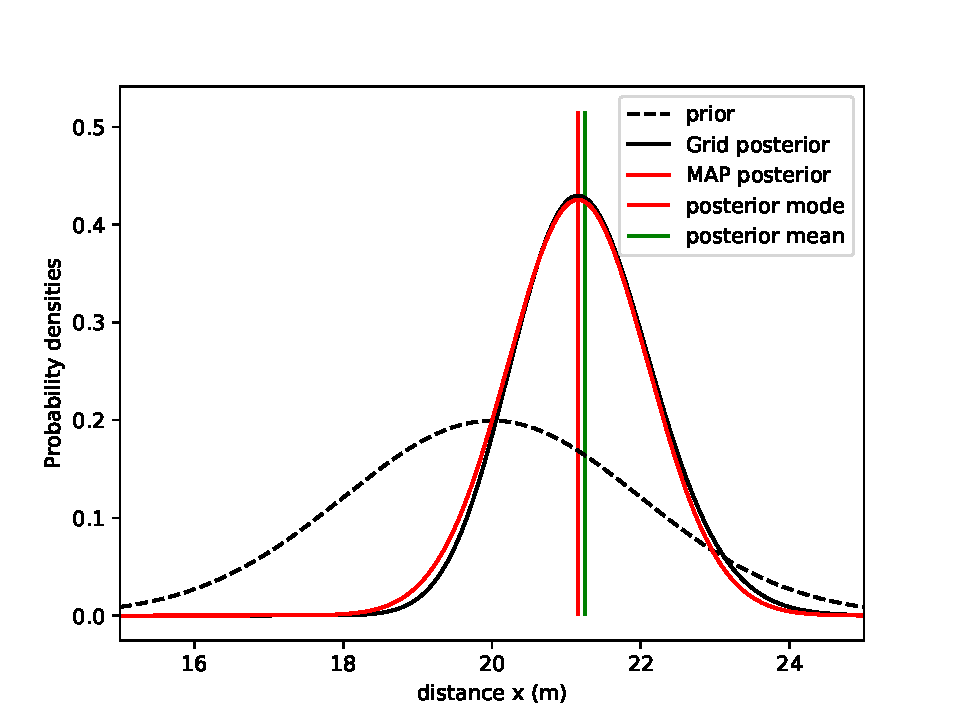
\includegraphics[width=0.9\textwidth]{figures/MAP_stereo1D.pdf}
    \caption{Representation of posterior inference on the toy problem. Dotted black: prior on $x$, 
    continuous black: numerical "grid" integration of the posterior, continuous red: Laplacian approximation of the posterior. Vertical lines: red=MAP, green=mean of the posterior
    }
    \label{fig:MAP_stereo1D}
 \end{figure}




\section{Lie groups for state estimation}
Some of the state variables that we manipulate in robotics are challenging since they do not belong to vector spaces. Some of the equations
involved in the Gauss-Newton algorithm, in particular the Gauss-Newton step update, cannot be be directly applied without extra care when it is the case.
These variables live on smooth manifolds, also known as Riemannian manifols. Many examples of Riemanian geometry in data science and robotics
\cite{miolane2020geomstats}. Besides, many of these robotics state variables also exhibit a group structure which, together with the smooth manifold
property, define the so called Lie group.
In this section we will provide the minimal concepts of smooth manifold and Lie groups that useful to the robotician. In particular, we will show 
that a limited number of notations can be made to the Gauss-Newton algorithm to accommodate for the special structure of these variables.

\subsection{Smooth manifold structure}
A \textit{smooth manifold} $\cM$ or differentiable manifold is a topological space that can be pictured as a smooth surface embedded in a higher dimensional vector space, 
of dimension $n$.
The smoothness property means that to each surface point $\bfx$ corresponds a unique tangent (hyper-)plane $\cT_{\bfx}\cM$, called the tangent space 
(there are no spikes or edges on the surface). The tangent space is a vector space on which traditional calculus operations are applicable. The dimension $m \leq n$ of this 
vector space is equal to the dimension of the surface as well as the degrees of freedom of its elements.
The element of tangent space at $\bf_x$, $\bftau\hhat \in \cT_{\bfx}\cM$ can naturally be decomposed as a linear combination 
of the tangent space basis vectors $E_i$. We can therefore define an element by its coefficient, which is the vector $\bftau \in \Reals^m$, called the cartesian tangent vector.
The \textit{hat} and \textit{vee} are mutually inverse linear maps permit to pass back and forth from $\cT_{\bfx}\cM$ to $\Reals^m$, which are therfore isomorphic:

\begin{align}
    \text{Hat} ~ :& \quad\quad \Reals^m \rightarrow \cT_{\bfx}\cM; \quad\quad \bftau \rightarrow \bftau\hhat = \sum_{i=1}^m\tau_i E_i  \\
    \text{Vee} ~ :& \quad\quad \cT_{\bfx}\cM \rightarrow \Reals^m; \quad\quad \bftau\hhat \rightarrow (\bftau\hhat)\vvee = \bftau = \sum_{i=1}^m\tau_i \bfe_i
\end{align}
where $\bfe_i$ are basis vectors of $\Reals^m$.

Vector spaces operations such as addition of a vector to a point or subtraction of two vectors do not apply in Riemannian geometry. For instance, if we
take a point on a sphere (the 2-sphere embedded in the 3 dimensional Euclidean space for instance) and add to it an arbitrary vector, we do not get in general
a another point on the sphere. These operations have equivalent in the \textit{retraction} and its inverse.
Retraction pulls an element from the local tangent space back to the manifold as represented in \figRef{fig:manifold}. We denote retraction and its inverse as 
$\oplus$ and $\ominus$:
%
\begin{align}
            \text{Retraction}~:&\quad\quad \bfx_2 = \bfx_1 \oplus \bftau   \\
    \text{Retraction inverse}~:&\quad\quad \bftau = \bfx_2 \ominus \bfx_1  \\
\end{align}
%
Note that we informally define the retraction and its inverse as operations dealing with the 
\begin{figure}[h]
    \centering
    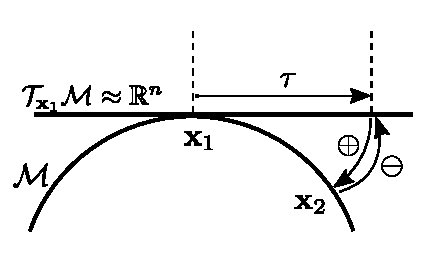
\includegraphics[width=0.7\textwidth]{figures/manifold.pdf}
    \caption{Manifold, tangent space, retraction and inverse retraction operation}
\end{figure}

When dealing with a collection of objects $\bfx_i$ living in their respective manifold $\cM^i$, it is often convenient to define a composite manifold
as the concatenation $\cM_c \triangleq \left<\cM^1, \dots, \cM^M \right>$. The element of this composite manifold is denoted by $\cX$
The composite equivalent of retract operation $\boxplus$ and 
its inverse $\boxminus$ retraction to individual elements of the manifold and its tangent space separately:

\begin{equation}
    \cX=
    \begin{bmatrix}
        \bfx^1 \\
        \vdots \\
        \bfx^M
    \end{bmatrix},
    \quad
    \cX \boxplus \bftau
    \begin{bmatrix}
        \bfx^1 \oplus \bftau_1 \\
        \vdots \\
        \bfx^M \oplus \bftau_M
    \end{bmatrix}
    \quad
    \cX_2 \boxminus \cX_1
    \begin{bmatrix}
        \bfx^1_2 \ominus \bfx^1_1 \\
        \vdots \\
        \bfx^M_2 \ominus \bfx^M_1
    \end{bmatrix}
\end{equation}



\subsection{Back to the MAP optimization problem}
Elements of the tangent space can be interpreted as steps that we can make to go from one point of the manifold to another.
This ties closely to the notion of Gaussian steps that we defined earlier. We will now consider that the estimated state $\cX$
is actually an element of a composite manifold (in which each state variables belongs to its own manifold). In this case, the Gaussian steps of \eqRef{eq:gaussian_step}
are in the composite manifold tangent space and the step updates writes:

\begin{equation}
    \check{\cX} := \check{\cX} \boxplus \Delta \bfx^*
\end{equation}

obtained by solving

\begin{equation}
    \Delta \bfx^* = \argmin_{\Delta \bfx} ||\bfr(\check{\cX} \oplus \Delta \bfx)||^2.
\end{equation}


Concerning residual formulation in \ref{eq:error_expectation}, if the measurement $\bfz_i$ is itself an element of a manifold, then the cartesian minus needs to be replaced:

\begin{equation}
    \bfe_i(\cX_{S_i}) = \bfh(\cX_{S_i}) \ominus \bfz_i,
    \label{eq:error_expectation}
\end{equation}

Note that many state variables actually belong to vector spaces (such as the robot position), which are trivial manifolds. For those, the $\oplus$ and $\ominus$ operators
simply reduce to the addition and subtraction of cartesian vectors.  



\subsection{Uncertainty in manifolds and jacobians}
Our state variables are random variables approximated by multivariate Gaussian distribution, that can be summarized by their mean vector and covariance matrix.
These concepts need to be slightly modified to account for the nature manifold nature of some of these. We will see how to define gaussian distribution on manifolds.
Let's $\tau \in \Reals^m$ be a small perturbation around a point $\bar{\bfx} \in \cM$, so that we can write:
%
\begin{equation}
    \bfx = \bar{\bfx} \oplus \bftau, \quad \bftau = \bfx \ominus \bar{\bfx}
\end{equation}
%
where $\bar{\bfx}$ designate the mean value of the distribution on $\bfx$. 
We actually define a zero mean "cartesian" gaussian distribution on the tangent space, the covariance being defined as:

\begin{equation}
    \Cov_{\bfx} = \mathbb{E}[\bftau\bftau^T] = \mathbb{E}[(\bfx \ominus \bar{\bfx})(\bfx \ominus \bar{\bfx})^T] \in \Reals^{m \times m}
\end{equation}
where $\mathbb{E}[\cdot]$ denotes the expectation operator.
By a slight abuse of notation, we note that the manifold distribution is $\bfx \approx \Gaussian{\bfx}{\Cov_{\bfx}}$

As an illustration, the group of unit quaternions $\mathbb{H} = \{ \bfq \in \Reals^4, \bfq \odot \bfq^*=1$ under quaternion multiplication $\odot$ is a manifold  
(the $S^3$ sphere, n=4 and m=3) \cite{sola2012quaternion}. 
The tangent space is the set of antisymmetric matrices, which is isomorphic to the angle axis rotation vectors $\angvel{}{} = \omega \bfu \in \Reals^3$.
If we naively define the covariance matrix of a quaternion as $\mathbb{E}[(\bfx \ominus \bar{\bfx})(\cX \ominus \bar{\cX})^T] \in \Reals^{4 \times 4}$, 
this covariance matrix is ill-defined. The covariance is instead defined as a $3 \times 3$ real matrix on the angle axis space.

In general, covariances can be propagated through nonlinear function of random variables using the chain rule. For instance, if $\bfx \in \Reals^{n_x}$ and 
$\bfy \in \Reals^{n_y}$ are cartesian multivariate gaussian distribution related by the nonlinear function $f$, propagating the $\bfx$ covariance 
$\Cov_{\bfx} \in \Reals^{n_x \times n_x}$ through f writes:

\begin{equation}
    f~: \bfx \in \Reals^{n_x} \rightarrow \bfy \in \Reals^{n_y}, \quad \quad \Cov_{\bfy} \approx 
                \left.\frac{D f}{D \bfx} \right|_{\bfx}   \Cov_{\bfx}    \left.\frac{D \bfy}{D \bfx}\right|_{\bfx}^T
\end{equation}

The same equation applies for random variables $\bfx \in \cM_{\bfx}$ and $\bfy \in \cM_{\bfy}$ living on manifolds. The definition of jacobians has however
to be redefined as:

\begin{equation}
    \frac{D f}{D \bfx} \triangleq \lim_{\bftau \to 0} \frac{f(\bfx \oplus \bftau) \ominus f(\bfx)}{\bftau}
\end{equation}

These jacobians also play a central role in the derivation of the residual jacobians \ref{eq:res_jacobian}.
Examples of manifold jacobian derivations in the context of Lie groups can be found in \cite{sola2018micro}.  



\subsection{Lie groups for robotic state estimation}
A \textit{group} ($\cG$, $\circ$) is a set $\cG$ with a composition law $\circ$ which satisfies the group axioms:

\begin{align}
    \text{Closure under}~'\circ'~:&~\bfx \circ \bfy \\ 
    \text{Associativity}~'\circ'~:&~(\bfx \circ \bfy) \circ \bfz = \bfx \circ (\bfy \circ \bfz) \\ 
    \text{Identity element}~\cE~:&~\bfx \circ \cE = \cE \circ \bfx = \bfx \\ 
    \text{Inverse}~\bfx^{-1}~:&~\bfx^{-1} \circ \bfx = \bfx \circ \bfx^{-1} = \cE
\end{align}
where, here, $\bfx,\bfy,\bfz \in \cG$.

Simply stated, a \text{Lie group} is a group which elements live in a smooth manifold $\cM$.

As a vector can represent a displacement from one point to an other along a straight line in the euclidean space or directly a point (displacement from the origin),
an element of a Lie group represents a path from one element to another along a geodesic of the manifold or directly an element of the group 
(displacement from the identity element $\cE$).

In particular the identity element $\cE$ relates to a notion of a global reference from which each element of the manifold can be compared.
The tangent space at this element is called the Lie algebra $\mathfrak{m} \triangleq \cT_{\cE}\cM$.

Let's compute the retraction operations in the case of Lie groups. We will follow the example of 3D rotations as they are of great use in robotics and provide good
good intuitions regarding the general behavior of Lie groups.
The group of 3D rotations is defined as the Special Orthogonal group in 3D: 
\begin{equation}
    \SO(3) = \left\{\Rot{}{} \in \text{GL}(n,\Reals) | \Rot{}{}\Rot{}{}^T=\Rot{}{}^T\Rot{}{}=I,~det(R)=1\right\}
\end{equation}
under matrix multiplication.


Firstly, properties that make $SO(3)$ a group are immediate from the:
%
\begin{itemize}
    \item Closure under the matrix product
    \item Associativity through the matrix product
    \item Identity element $\bfI_3$
    \item Inverse element $\Rot{}{}^{-1} = \Rot{}{}^T$ (from the group definition)
\end{itemize}
%
Let's explicit the manifold structure of $\SO(3)$. First, the topology of its corresponding manifold is the $S^3$ sphere.
It can be showed \cite{sola2018micro} that taking the time difference of a rotation matrices results in an element of its local tangent space
$\dot{\Rot{}{}} = \Rot{}{} [\angvel{}{}]_{\times} \in \cT_{\Rot{}{}}\SO(3)$ where $[\angvel{}{}]_{\times}$ is the skew-symmetric operator associated to the cross product. 
$[\angvel{}{}]_{\times} = \angvel{}{} \times \cdot$. The Lie algebra $\so(3)$ is therefore the 3 dimensional vector space of antisymmetric matrices. 
For a constant $\angvel{}{}$, this defines an ordinary differential equation (ODE) whose solution
is $\Rot{}{}(t)=\Rot{}{0}\exp([\angvel{}{}]_{\times}t)$ where exp is the matrix exponential:

\begin{equation}
    \exp(\bfA) = \sum_{k=0}^{\infty} \frac{\bfA^k}{k!}
\end{equation}

For $\SO(3)$ and most other Lie groups, properties of the Lie algebra simplifies the infinite sum of the matrix exponential to a simpler closed form formula. 
In the $\SO(3)$ case, this formula is known as the Rodriguez equation:

\begin{equation}
    \Exp(\bftheta) = \exp([\bftheta]_{\times}) = \bfI + [\bfu]_{\times}\sin(\theta) + [\bfu]_{\times}^2(1 - \cos(\theta))
\end{equation}
where $\bftheta \triangleq \theta \bfu \in \Reals$ where $\theta$ is the norm of the rotation vector, which is an angle (in radians).
Finally, we have denoted by $\Exp$ the composition of the $hat$ operator ($\bftheta\hhat \triangleq [\bftheta]_{\times}$). 
The inverse operation that maps elements from the group to the Lie algebra is defined as the $\Log$ map. A general representation of
Lie group operation can be found in \figRef{fig:lie_group}

We all of that in mind, the link with the Riemannian manifold terminology becomes clearer. We can compose a rotation with
an increment $\angvel{\bfx}{}$ taken in the tangent space at $\bfx$ to obtain another rotation: $\Rot{}{2} = \Rot{}{1}\Exp(\angvel{}{12})$.
This corresponds to the $\oplus$ retraction operator. Conversely, the inverse of the retraction $\ominus$ corresponds to the application of The
logarithm on the relative rotation as described here:

\begin{align}
    \Rot{}{2} &= \Rot{}{1}\oplus \angvel{}{12} = \Rot{}{1} \Exp(\angvel{1}{12})  \\ 
    \angvel{1}{12} &= \Rot{}{2}\ominus \Rot{}{2} = \Log(\Rot{}{1}^T\Rot{}{2}) 
\end{align}

\begin{figure}[h]
    \centering
    \begin{subfigure}{0.85\textwidth}
        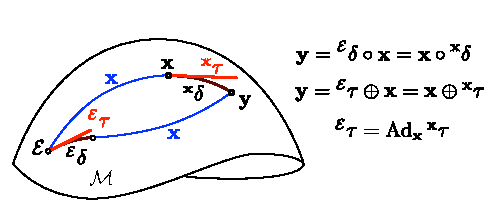
\includegraphics[width=\textwidth]{figures/lie_group.pdf}
        \caption{Representations of a Lie group including the identity element $\cE$, operations of composition
        between increments and relations between a tangent space increment at the identity $\prescript{\cE}{}{\bftau}$ 
        and at the local element $\prescript{\bfx}{}{\bftau}$ through the adjoint matrix $\text{Ad}_{\bfx}$. Figure adapted from \cite{sola2018micro}.}
        \label{fig:lie_group} 
    \end{subfigure}

    \begin{subfigure}{0.85\textwidth}
        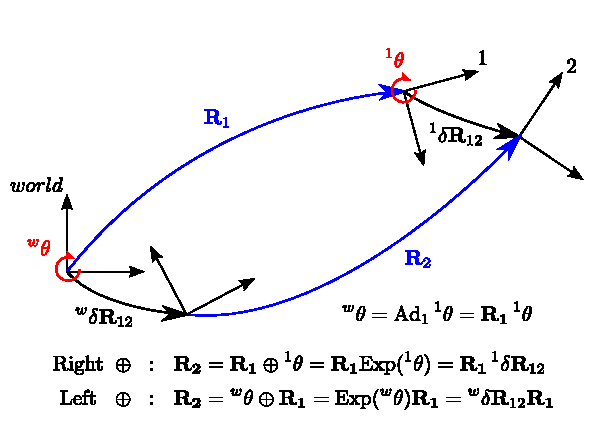
\includegraphics[width=\textwidth]{figures/rotation_exp_log.pdf}
        \caption{Representation of $\SO(3)$ Lie groups operations. Note that we represented frames with different origins
        for better readability while the group elements only represent pure rotations (no translation).}
        \label{fig:rotation_exp_log} 
    \end{subfigure}
\end{figure}

In robotics terms, $\angvel{1}{12}$ is the axis angle representation of the relative rotation $\delta \Rot{1}{12} = \Rot{}{1}^T\Rot{}{2}$ and
\textit{local} rotations represent the orientation of reference frames in a \textit{global} world reference frame. The identity element therefore corresponds 
to the world frame. For Lie group, an additional $\oplus$ operator exists which retracts and compose vectors at the Lie algebra instead of
the local algebra, the left-$\oplus$ while the local one is called the right-$\oplus$. The Adjoint $\text{Ad}_{R}\SO(3)$ is a linear operator that permits to map
elements from the local tangent space to the Lie algebra. Those operations are illustrated by \figRef{fig:rotation_exp_log}.


%
%
%
\section{Factor graphs: a visual language for robotics estimation}
A crucial aspect of solving the MAP problem is the factorizibility of the likelihood function. This represents the fact that the problem
exhibits a particular structure that has important computational implications. We will first explain how this factorization can be described 
visually using a graphical model known as the \textit{Factor Graph} and then link this representation to the sparsity of the matrix involved
in solving the NLLS problem.


\subsection{Factor Graph representation}
Let's consider the toy example represented in \figRef{fig:toy_problem}. 
We wish to estimate the trajectory of a differential robot, that is its states at chosen timestamps called \textit{\keyframes}, and \textit{landmarks} which are elements of the 
environment that are easily detectable. We suppose that this robot is equipped with an odometer, which measurements integrated over time provide relative 
transformations between \keyframes, and an exteroceptive sensor, which provides relative measurements between \keyframes~and landmarks.

\begin{figure}[h]
    \centering
    \begin{subfigure}{.49\linewidth}
        \centering
        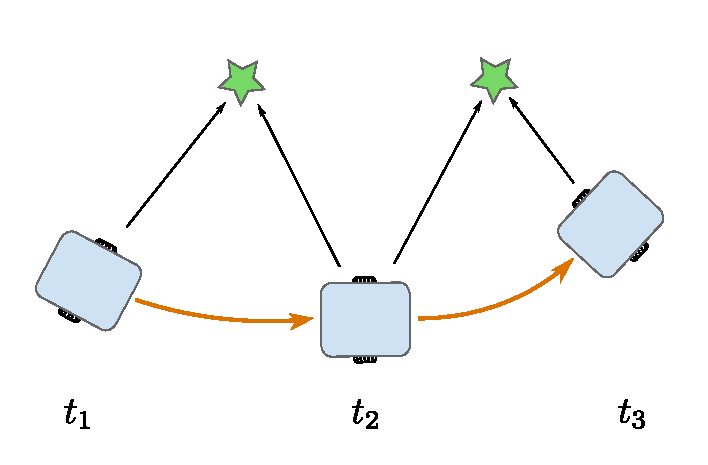
\includegraphics[width=\textwidth]{figures/toy_example.pdf}
        \caption{\label{fig:toy_problem}}
    \end{subfigure}%
    \hfill
    \begin{subfigure}{.49\linewidth}
        \centering
        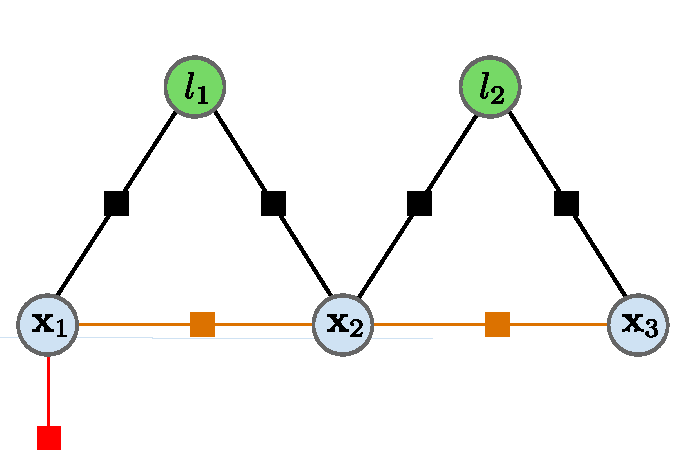
\includegraphics[width=\textwidth]{figures/toy_factor.pdf}
        \caption{\label{fig:toy_factor}}
    \end{subfigure}%
    \caption{(\subref{fig:toy_problem}): toy estimation problem, a differential drive robot equipped with an odometer moves in 
    an scene with landmarks represented by stars. \subref{fig:toy_factor}): factor graph representation the problem, the estimated variables are represented by circles 
    (blue for robot \keyframe, green for landmarks) and factors by squares (orange for odometry, black for exteroceptive sensor, red for the prior).}
\end{figure}

In this case, the state variables are $\cX = \{ \bfx_1, \bfx_2, \bfx_3, l_1, l_2\}$ 
and measurements $\cZ = \{ z_{o,1}, z_{o,2}, z_{e,1}, z_{e,2}\}$
We also apply a prior on the pose of the first \keyframe of the trajectory, which can be understood as fixing the frame origin of the reference 
frame in which the estimation is done.

The factorization of the likelihood of \eqRef{eq:likelihood_factorization} in this example writes:
%
\begin{align}
    p(\cX | \cZ) \propto 
    ~&{\color{Red} \phi_0({\color{Blue} \bfx_{0}})} \\ 
    ~&{\color{Orange} \phi_1({\color{Blue} \bfx_1}, {\color{Blue} \bfx_2}) \phi_2({\color{Blue} \bfx_2}, {\color{Blue} \bfx_3})} \\ 
    ~&{\color{Black} \phi_3({\color{Blue} \bfx_1}, {\color{Green} l_1}) \phi_4({\color{Blue} \bfx_2}, {\color{Green} l_1}, {\color{Green} l_2}) \phi_5({\color{Blue} \bfx_3}, {\color{Green} l_2})} \\ 
\end{align}
%
This factorization can be represented as a \textit{factor graph} as seen in \ref{fig:toy_factor}. 
factor graphs are popular graphical models \cite{koller2009probabilistic} that can describe a vast family of statistical models \cite{loeliger2004introduction}.
A factor graph in the most general sense is a bipartite graph that represents the factorization of a function of several variables. 
We adopt the visual notation commonly found in robotics: round nodes for variables, square nods for factors, edges represent the dependency 
of each factor on a subset of variables. Over the last two decades, they have grown in popularity among roboticists as a visual language to describe 
estimation problems \cite{dellaert2017factor} and planning problems \cite{dong2016motion}. Dellaert and Kaess \cite{dellaert2006square} were the first to
recognize the link between NLLS problems and factor graph.

% Many specialized solvers \cite{grisetti2011g2o, dellaert2012factor, ila2017slam++} have been implemented that exploit the sparse structure of these 
% problems. A discussion of the particularities of factor graph-based NNLS solvers can be found in \cite{dellaert2017factor, sola2017course}.

\subsection{Sparsity of the NLLS problem}

The jacobian matrix of the residuals $\bfJ \in \Reals^{M \times N}$ is a big sparse matrix of dimensions 
\begin{itemize}
    \item N columns = $\sum_{i=1}^{n}dim(\cT_{\bfx_i}\cM_i)~\rightarrow$ the sum of variables tangent spaces dimensions 
    \item M rows = $\sum_{i=1}^{m}dim(\bfe_i) \rightarrow~$ the sum of residual dimensions
\end{itemize}   

Each block column corresponds to one of the state variables and each row corresponds to a residual.
\begin{equation}
    \bfJ=
    \begin{pmatrix}
       J^{p}_{\bfx_1} &   &     &     &     \\
       J^{o_1}_{\bfx_1} & J^{o_1}_{\bfx_2}  &     &     &     \\
                       & J^{o_2}_{\bfx_2}  & J^{o_2}_{\bfx_3}   &     &     \\
       J^{e_1}_{\bfx_1} &                  &     &  J^{o_2}_{\bfl_1}   &     \\
                       & J^{e_1}_{\bfx_2}  &     &  J^{e_1}_{\bfl_1}   &     \\
                       & J^{e_2}_{\bfx_2}  &     &     &  J^{e_2}_{\bfl_2}   \\
                       &                  & J^{e_3}_{\bfx_3}    &     &  J^{e_3}_{\bfl_2}   \\
    \end{pmatrix}
    \label{eq:sparse_jac}
\end{equation}

The approximate hessian matrix $\bfH \in \Reals^{N \times N}$ displays a similarly remarkable sparsity which makes the resolution of the linear system
at each step very efficient. Algorithms such as the Schur complement, Cholesky factorization and QR factorization were applied by different authors to the 
problem of SLAM and estimation.








% CONCLU